
\section{Exploratory Analysis}
\label{sec:background}

We first performed a 6:1 train/test split on our data, giving us a dataset of 60000 images for the training data and 10000 images for the testing. This will allow us to test the model with data not seen in training to give us a true test of the accuracy. If the model over-fits our training data, this will show in the testing results, as it will not perform as well on unseen data.

One interesting aspect of the dataset is that some categories are very similar - so much so that an untrained human might have a hard time distinguishing between the two. Most notably, T-shirt/top and shirt are extremely similar categories. Secondly, pullover and coat also might be tricky to distinguish in some cases. We expect that the model might have a harder time distinguishing between these categories, especially because the 28x28 pixel images are low resolution and therefore might not be able to convey some distinctions (for example a pullover and a coat might look similar with the zipper as the exception). Figures 1 and 2 display what the 28x28 image looks like. As you can see, it would be difficult for a human to categorize these two shirts given the different labels which leads us to believe the model will also have a hard time distinguishing them, as the outline is consistent across both categories. By definition, the difference between a T-shirt and a shirt is material, which would be hard to distinguish given the low resolution image.


\begin{figure}[!h]
    \centering
    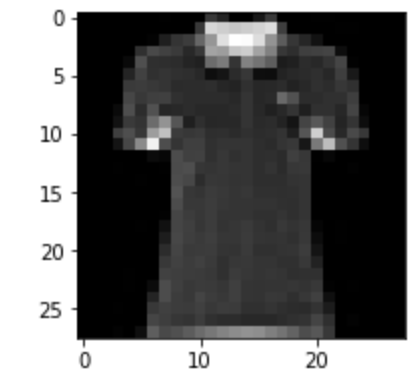
\includegraphics{label0.png}
    \caption{Shirt with corresponding label=0 "T-shirt/top"}
    \label{fig:label0}
\end{figure}

\begin{figure}[!h]
    \centering
    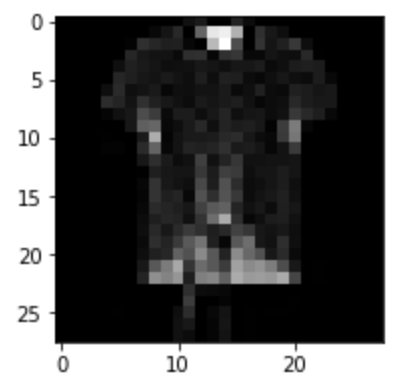
\includegraphics{label6.png}
    \caption{Shirt with corresponding label=6 "Shirt"}
    \label{fig:my_label}
\end{figure}






